\documentclass[journal,12pt,twocolumn]{IEEEtran}
\usepackage{amsmath,amssymb,amsfonts,amsthm}
\usepackage{txfonts}
\usepackage{tkz-euclide}
\usepackage{listings}
\usepackage{gvv}
\usepackage[latin1]{inputenc}
\usepackage{array}
\usepackage{pgf}
\usepackage{lmodern}
\usepackage{amsmath}
\usepackage{circuitikz}
\begin{document}
\bibliographystyle{IEEEtran}

\title{GATE 2022[IN]-64}
\author{EE23BTECH11066 - Yakkala Amarnath Karthik}
\maketitle
\bibliographystyle{IEEEtran}

\textbf{Question:}\\
In the circuit shown, the switch is initially closed. It is opened at t= 0 s and
remains open thereafter. The time (in milliseconds) at which the output voltage
$V_{out}$ becomes LOW is  (round off to three decimal places

\begin{figure}[ht]
    \centering
    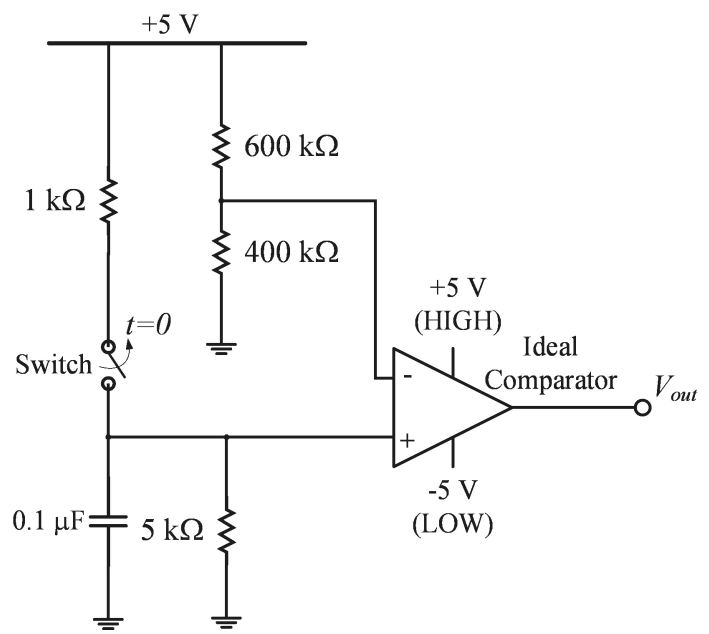
\includegraphics[width=0.45\textwidth]{figs/circuit question.png}
    \caption{circuit diagram}
\end{figure}


\textbf{Solution:}\\
At t$=0^-$, when the switch is closed,\\
The voltage across the capacitor is:
\begin{align}
V_c\brak{0^-}&=5*\frac{5}{5+1}\\
&=\frac{25}{6}V
\end{align}
$V_c\brak{0^-}$ is also the non inverting voltage of the OP-AMP\\ \\
At $t=0^+$, when the switch is open,\\
The voltage across inverting terminal is:
\begin{align}
V_I&=5*\frac{600}{600+400}\\
&=2V
\end{align}
Immediately after the switch is open, voltage across capacitor do not change.\\ So $V_{NI}>V_I$,Hence the output of OP-AMP is fixed to 5V.
Later, Capacitor discharges into 5K$\Omega$ resistor.\\
The discharging equation is as follows:
\begin{align}
    V_C\brak{t}&=V_C\brak{0^-}e^{\frac{-t}{\tau}}\\ 
    2&=\frac{25}{6}*e^{\frac{t_0}{RC}}\\
    t&=RC\ln\brak{\frac{25}{12}}\\
    &=0.1*10^{-6}*5*10^{3}\ln{\brak{\frac{25}{12}}}\\
    t&=0.367 ms
\end{align}

\begin{figure}
\centering
\begin{circuitikz}

    % Draw resistors and voltage source
    \draw (0,0) node[left] {$5V$}to[resistor={{$600\Omega$}}] (2,0) ;
    \draw (2,0) -- (2,-1) to[resistor={{$400\Omega$}}] (0,-1) node[ground]{};
    \draw (2,-0.5) --(3,-0.5) -- (3,-2.5);
    
    \draw (5,-3) node[op amp] (opamp) {};
    \draw (opamp.up) ++(0,0.3) node[above] {$+5V$};
     \draw (opamp.down) ++(0,-0.3) node[below] {$-5V$};
    \draw (opamp.-) -- (3,-2.5)node[left]{$V_I=2V$};
    \draw (opamp.out) -- (6,-3) --(7,-3) node[right] {$V_{out}$};
    \draw (opamp.+) -- (3,-3.5)node[left]{$V_{NI}$} -- (3,-4.5);
    \draw (3,-4.5) to[resistor={{$5k\Omega$}}] (3,-6.5)node[ground]{};
    \draw (3,-4.5) -- (0.8,-4.5);
    \draw (0.8,-4.5) to[C, l=$0.1\mu F$] (0.8,-6.5)node[ground]{};
\end{circuitikz}
    \caption{circuit diagram at $t=0^+$};
\end{figure}


\end{document}
